	\documentclass[12pt]{article}
\usepackage{xeCJK}

\usepackage{charter}
\usepackage{fullpage}
\usepackage[colorlinks=false]{hyperref}
\usepackage{ifthen}
\usepackage{comment}
\usepackage[title,titletoc]{appendix}
\usepackage{pagecolor}
\usepackage{amsmath}
\usepackage{amsfonts}
%\usepackage[normalem]{ulem}
\usepackage{siunitx}
\usepackage{amsthm}
\sisetup{per=slash, load=abbr}
\usepackage{paralist}
\usepackage{pgfplots}
\usetikzlibrary{positioning}
\usetikzlibrary{fit}
\usetikzlibrary{snakes}
\usetikzlibrary{shapes.geometric}
\usetikzlibrary{patterns}
\usetikzlibrary{shapes,arrows,chains}
\usepgfplotslibrary{patchplots,colormaps}
\usetikzlibrary{calc}
\usetikzlibrary{positioning, fit}
\usetikzlibrary{backgrounds}
\usetikzlibrary{intersections}

\newcommand{\whitepaper}[1]{\begin{center}\fbox{\parbox{0.75\textwidth}{{\small
#1}}}\end{center}}

\newcommand{\pcolor}{violet!25}

\usepackage{setspace}
\usepackage{algorithm2e}
\bibliographystyle{ieeetr}

\usepackage{geometry}
\geometry{left=3cm,right=3cm,top=1.6cm,bottom=3cm,headheight=0pt,headsep=1.5em}
\usepackage{fancyhdr}
\pagestyle{fancy}
\chead{
\includegraphics[scale=0.2]{../common/Nebulas.png}}  %在此处插入logo.pdf图片 图片靠左
\lhead{} % 页眉中间位置内容
\rhead{}
\usepackage{expl3}
\ExplSyntaxOn
\newcommand\latinabbrev[1]{
  \peek_meaning:NTF . {% Same as \@ifnextchar
    #1\@}%
  { \peek_catcode:NTF a {% Check whether next char has same catcode as \'a, i.e., is a letter
      #1.\@ }%
    {#1.\@}}}
\ExplSyntaxOff

%Omit final dot from each def.
\def\eg{\latinabbrev{e.g}}
\def\etal{\latinabbrev{et al}}
\def\etc{\latinabbrev{etc}}
\def\ie{\latinabbrev{i.e}}
\newcommand{\dapp}{DApp\xspace}

%\setlength{\topskip}{1em}

\usepackage{indentfirst}

%\usepackage{algorithm}
\usepackage{algpseudocode}
\usepackage{amsmath}
\usepackage{amsfonts}
\usepackage{amssymb}
\renewcommand{\algorithmicrequire}{\textbf{Input:}}  % Use Input in the format of Algorithm
\renewcommand{\algorithmicensure}{\textbf{Output:}} % Use Output in the format of Algorithm



\setCJKmainfont[BoldFont = STSongti-SC-Bold]{STSongti-SC-Regular}
\setCJKfamilyfont{hei}{SIL-Hei-Med-Jian}		%宋体
\setCJKfamilyfont{song}{SimSun}		%宋体
\setCJKfamilyfont{kai}{Kaiti}		%楷体
\setCJKfamilyfont{fang}{song}	%仿宋
\setCJKfamilyfont{li}{song}			%隶书
\setCJKfamilyfont{you}{Yuanti}		%幼圆

\newcommand{\song}{\CJKfamily{song}}	%宋体
\newcommand{\hei}{\CJKfamily{hei}}	%黑体
\newcommand{\kai}{\CJKfamily{kai}}	%楷体
\newcommand{\fs}{\CJKfamily{fang}}	%仿宋
\newcommand{\li}{\CJKfamily{li}}		%隶书
\newcommand{\you}{\CJKfamily{you}}	%幼圆
\newcommand{\reffig}[1]{图\ref{#1}}
\newcommand{\refsec}[1]{\S \ref{#1}}

\onehalfspacing   % ----------设置1.5倍行距(可能有意义,待调整)

%\parindent=20pt  % -------------------首行缩进大小,英文分段就直接0pt了吧。
\setlength{\parindent}{2.1em}
\setlength{\parskip}{0.3\baselineskip}
\newcommand{\nrcore}{Core Nebulas Rank}
\newcommand{\nrext}{Extended Nebulas Ranks}
\newcommand{\dom}{{\; \texttt{dom}\;}}
\newcommand{\nr}{\Gamma}

\setCJKsansfont[BoldFont = STHeitiSC-Medium]{STHeitiSC-Light}


\newtheorem{property}{特征}
\newtheorem{corollary}{推论}
\newtheorem{definition}{定义}
%\addbibresource{reference.bib}

\begin{document}
\pagestyle{empty}
\renewcommand{\contentsname}{目录}
\renewcommand{\abstractname}{摘要}
\renewcommand{\refname}{参考文献}
%\renewcommand{\nomname}{术语表(按首字母排序)}
\renewcommand{\figurename}{图}
\renewcommand{\tablename}{表}
\renewcommand{\baselinestretch}{1.5}
\renewcommand{\appendixname}{附录}
\renewcommand{\proofname}{证明}

%\pagecolor{\pcolor}

\begin{titlepage}
  \begin{center}
    \vspace*{5.5cm}
    
\includegraphics[scale=0.5]{../common/Nebulas.png}
    \vspace{0.5cm}


   \textbf{\huge{共识机制设计指导}}

    \vspace{0.5cm}
    星云研究院
    \vfill
    2019年3月 \\
    版本号:0.0.1
    \textbf{}
  \end{center}

\end{titlepage}
\setcounter{page}{0}
%\thispagestyle{empty}

\tableofcontents
\newpage
\setcounter{page}{1}
\pagestyle{fancy}
\vspace*{0.01cm}
% !TEX root = main.tex
\section{简介}
共识(Consensus)是布式系统中的基本性质之一,具体来说是指通过消息传递使得系统中所有节点均以相同顺序执行一个命令序列\cite{lamport1978implementation}。而在实际环境中,节点可能出错产生异常行为,或者消息无法被正确传递,使得系统无法达成一致\cite{pease1980reaching}。早期研究指出,当系统中仅有两个节点时,不存在一种容错协议使得系统达成一致\cite{akkoyunlu1975some}。1982年Lamport等人将其扩展为多节点下的容错问题,即拜占庭将军问题(Byzantine Generals Problem,BGP)\cite{lamport1982byzantine}。

拜占庭将军问题被认为是容错性问题中最难的问题类型之一,在区块链技术出现之前,拜占庭容错并没有得到广泛关注。自上世纪90年代起,由Lamport提出的Paxos算法\cite{lamport2001paxos}被公认为分布式系统共识的经典解决方案\cite{chandra2007paxos},并得到了广泛的应用\cite{burrows2006chubby,chang2008bigtable,ghemawat2003google}。但Paxos等算法仅能实现宕机容错(Crash-Fault Tolerant)而不满足拜占庭容错(Byzantine-Fault Tolerant)。

2008年匿名发布的比特币白皮书\cite{nakamoto2008bitcoin}提出了一种去中心化的账簿,其从全新的角度阐述了拜占庭环境下的共识解决思路。以比特币为代表的区块链也属于分布式系统,由于存储在这些帐簿中的价值,恶意节点有巨大的经济动机去尝试造成故障,因此这类分布式系统对于拜占庭容错的需求非常高\footnote{Understanding Blockchain Fundamentals, https://medium.com/loom-network/understanding-blockchain-fundamentals-part-1-byzantine-fault-tolerance-245f46fe8419}。

区块链技术的出现让拜占庭容错问题重新得到关注,而尝试解决拜占庭容错问题的共识算法也不断被提出。早期的区块链共识机制与传统的拜占庭容错算法存在较大差异,例如比特币中通过算力竞争的方式决定出块权,并且基于最长链原则实现了大规模节点的状态同步\cite{nakamoto2008bitcoin}。近几年出现了许多结合经典分布式系统BFT机制的共识机制,例如Tendermint\cite{buchman2016tendermint}、Byzcoin\cite{kogias2016enhancing}等等。


%此类问题被定义为拜占庭容错(Byzantine Fault Tolerant,BFT)问题\cite{pease1980reaching}。进一步地,论文\cite{lamport1982byzantine}给出了
%,共识被定义为状态机复制(State Machine Replication),即对于所有。
%而当存在恶意节点的情况下,共识被描述为拜占庭容错问题(Byzantine Fault Tolerant,BFT)。



%大多数BFT算法实际上在尝试解决拜占庭将军问题(Byzantine Generals Problem,BGP),即拜占庭容错问题的一个特例。

%传统分布式服务中\cite{castro1999practical},
%领导者的选取由发起请求的客户端(client)指定或者由固定算法决定(例如$mod\ n$),


实际上,区块链系统的共识机制涉及到众多领域,包括密码学、分布式系统甚至是经济学等。各种区块链共识算法,其实现机制千差万别,究其原因是其设计者的研究背景各异以至于对区块链共识有着不同的理解\footnote{https://zhuanlan.zhihu.com/p/52251671}。因此在设计出合理的共识机制之前,我们需要回答如下问题:

\begin{itemize}
	\item 区块链共识机制需要解决什么样的问题?
	\item 理想的区块链共识机制需要满足什么样的要求?
\end{itemize}

在此,我们可以先回答第一个问题。

 作为广义上的分布式系统,区块链的共识也是为了解决拜占庭容错问题。对应到区块链的流程上通俗地来说,共识协议是在解决\textcolor{red}{“谁负责出块”和“出现分叉如何解决”}这两个问题\cite{ultrain2019},论文\cite{gilad2017algorand}将这两步定义为区块提议(Block Proposal)和一致达成(Agreement)。尽管许多共识机制并未对两者进行严格划分,但这种解耦思想有助于我们理解区块链共识并且在此基础上设计合理的共识算法\cite{kogias2016enhancing,eyal2016bitcoin}。

%一些研究将上述两个问题定义为\textcolor{red}{领袖选举(Leader Election)}和\textcolor{red}{交易验证(Transaction Verification)}\cite{kogias2016enhancing,gilad2017algorand,eyal2016bitcoin}。
%尽管在有些研究中两者没有被严格划分并且存在相关性\cite{gilad2017algorand},但将领袖选举和交易验证解耦
本文的后续章节则尝试回答第二个问题。

第二章简单介绍现有的区块链共识工作;第三章给出了区块链共识涉及到的系统模型;在此基础之上,第四章和第五章分别给出共识协议中区块提出和一致达成的性质分析。

需要注意,本文仅针对区块链共识机制提供设计指导,而并非完整的共识机制设计方案。

%本文旨在简单介绍区块链共识问题,尤其是领袖选举和交易验证,在此基础上给出相应的分析,从而为后续的共识设计提供指导。

%即拜占庭容错问题(Byzantine Fault Tolerant,BFT)\cite{pease1980reaching}的特例。
%通常针对BGP的算法往往。


% !TEX root = main.tex
\section{相关研究}
本章节简单介绍了已有的区块链共识研究工作,这里并未按照一些公认的划分方法\footnote{很多研究通常会将共识划分为PoW、PoS等等。},而是根据上述共识流程进行进行介绍。更详细的介绍可以参见星云共识调研报告[]。

\subsection{领袖选举}
相比于传统分布式系统,在匿名和去中心化场景下区块链共识的领袖选举需要应对更多挑战。同时,由于区块链系统对于节点的设定不同,其采领袖选举机制也不尽相同。

%为保证匿名性,区块链中所有节点均表示为基于公钥产生的地址(例如以太坊中长度为64位的16进制字符串),
%同时为保证去中心化以及防止DDoS攻击,客户端产生的transaction会更新到全节点共享的交易池中(transactions pool)而无法指定特定的节点来发起提案(proposal)[]。
以比特币\cite{nakamoto2008bitcoin}和以太坊\cite{wood2014ethereum}为代表的区块链对于出块节点(即领袖)没有准入限制,参与领袖选举的节点可以随时加入离开整个网络,此类区块链系统称之为无授权区块链(Permissionless Chain)。这类系统通过节点竞争方式选举领袖,其中最为广泛采用的算法是工作量证明(Proof-of-Work,PoW)。需要指出的是,PoW仅仅实现了领袖选举,而并不是完整的共识协议,这一点在比特币白皮书上已经指出\cite{nakamoto2008bitcoin},而一种普遍的错误是将PoW和比特币共识(通常称之为Nakamoto Consensus)混为一谈。

对于联盟链(Consortium Blockchain)以及部分采用DPoS机制的公链\cite{grigg2017eos},参与节点需要通过授权并且不能随意加入离开,因此被定义为授权区块链(Permissioned Chain)。在此类系统中,一段时间内所有参与节点集合已知且不变,领袖选举可以采用简单的轮询机制(Round-Robin)[]。从而整个共识问题退化成传统分布式系统中的共识问题,即在领袖选择已经达成共识的情况下(此时领袖仍可以采取恶意行动),所有验证节点如何针对领袖的提案(出块)达成一致。

目前关于授权区块链是否能称之为区块链尚存在争议\footnote{EOS is not a blockchain, https://thenextweb.com/hardfork/2018/11/01/eos-blockchain-benchmark/},但可以肯定的一点是,无授权区块链更符合去中心化思想。不断有研究尝试解决无授权环境下的领袖选举问题。

由于PoW会消耗大量电力,权益证明(Proof-of-Stake,PoS)随后被提出,不同于PoW,后者实现选举往往与链上资产相关而不依赖于物理算力因此都称之为PoS,但不同基于PoS的共识之间通常差别较大。早期的PoS仍然是基于PoW的变种实现\cite{king2012ppcoin},即对谜题计算中的目标基于权益(Stake)或币龄(Coin-age)进行加权。作为备受瞩目的以太坊演进方案,Casper\cite{buterin2017casper}被认为是一种PoS协议,但实际上Casper是利用stake实现链式结构的终结性(Finality),并不涉及领袖选举过程,后者仍然可以选择采用PoW机制。

无授权区块链对于参与节点没有身份验证,因此对于领袖选取需要引入随机性,以保证安全\cite{pass2017rethinking}。近几年涌现出一些基于随机数生成(Random Number Generation,RNG)的共识机制实现了非PoW领袖选举方案\cite{gilad2017algorand,david2018ouroboros,hanke2018difinity}。尽管在出块方式和共识实现上存在区别(例如Ouroboros基于弱同步时钟),上述方案均利用伪随机函数(pseudo-random function)实现了领袖的随机选举。

%同时根据[]的研究,在网络传输带宽有限的情况下,区块产生间隔和链分叉率存在相关性,因此在采用最长链等结构的区块链中,我们认为出块者选举机制也需要控制全网出块频率。

\subsection{交易验证}
\label{subsec:intro_tx_verification}
在分布式系统中,状态机复制可以有效解决多服务器之间的数据一致性问题\cite{schneider1990implementing}。最为经典的Paxos协议实现了宕机容错(crash-fault tolerant)的一致性算法\cite{lamport2001paxos},其被广泛应用于数据库备份和域名服务等领域\cite{burrows2006chubby,chang2008bigtable}。

随着区块链和数字货币的发展,基于拜占庭容错的一致性算法重新得到关注。在大规模节点网络中,网络通信成为瓶颈。以Bitcoin为代表的permissionless chain采取了最长链原则(Longest Chain Rule)\cite{nakamoto2008bitcoin},\cite{sompolinsky2015secure}提出了最重子树原则(GHOST Rule)。最长链和GHOST协议通常被称之为链式协议(chain-based Protocols),链式协议中节点仅依据接收区块构建链结构实现一致性而不产生额外的状态同步开销。对应地,链式协议仅能保证最终一致性(Eventual Consistency),即保证所有节点最终就共享状态达成一致,但在某个时间段内,共享状态各个节点所存的状态可能不一致。

联盟链以及部分公链通过缩小节点规模,实现了更强的一致性保证。节点针对每个提案进行投票,通常基于PBFT\cite{castro1999practical}或者更为宽松的投机BFT算法\cite{kotla2007zyzzyva},此类机制被称之为投票协议(vote-based Protocols)。相比于链式协议,投票协议对系统要求更为严格,PBFT和最差情况下的投机BFT网络通信开销为$O(n^2)$,因此采用此类协议的网络往往规模较小。

基于PBFT机制,ByzCoin\cite{kogias2016enhancing}利用集体签名(Collective Signing)实现了投票节点规模可扩展,因而在一些分片技术(sharding)中也被采用\cite{kokoris2018omniledger}。

采用投票协议的区块链会针对每个出块进行一致性确认,因此每个区块状态不可能被扭转,从而实现终结性(Finality)。相比之下,基于链式结构的区块链在达到最终一致性前任何区块状态都可能发生改变(例如某个区块在某个时间后不再属于最长链),通常这种改变概率随着链式结构增长单调递减\cite{nakamoto2008bitcoin},因此链式结构共识无法保证终结性,或者仅提供概率终结性(Probabilistic Finality)。较为特殊地,Casper\cite{buterin2017casper}在检查点(checkpoints)内部采用最长链原则,而不同检查点间则通过投票保证终结性。

需要指出的是,通常认为采用链式协议的系统吞吐量(Throughput)低于基于投票协议的系统,实际上在仅满足最终一致性条件以及同等节点规模和网络环境下,链式协议实现状态同步开销更低。

%Bitcoin和Ethereum的成功表明最终一致性能够满足去中心化交易和图灵完备编程需求,








% !TEX root = main.tex
\section{系统模型}
本章节主要给出区块链共识涉及到的相关定义,在此基础之上我们给出相关的评价指标。

\subsection{网络模型}
分布式系统中,节点之间的通信方式主要为消息传递(Message Passing)。根据网络传输延迟的设定,可以将系统划分为同步网络(Synchronous Network)和异步网络(Asynchronous Network)。在同步网络模型下,所有节点的消息传输延迟不会超过某个阈值;而在异步网络中,节点间的消息传输延迟可以是任意值。\textcolor{blue}{根据FLP定理[],异步网络环境下,只要存在一个拜占庭节点则BGP问题无解。}

一种看法是,由于实际网络一定存在传输延迟,因此不存在能够在能够保证容错的共识算法。客观来看,该观点没有错误,但过于悲观。目前所有拜占庭容错的共识算法均是基于同步网络模型,一些更为宽松的模型允许网络中除领袖以外节点之间的通信可以为异步网络,后者称之为“弱终止假设”(或“半异步网络”)\cite{castro1999practical}。在本文中,我们基于同步网络模型讨论共识算法。

\subsection{时钟模型}

由于网络传输延时,分布式系统中的节点无法实现完美同步时钟(Perfectly Synchronized Clock)\footnote{更本质的原因是,即便不存在网络延迟,由于相对论的存在也不可能实现完美同步时钟。}。一种更严谨的描述方法是采用逻辑时钟(Logical Clocks)\cite{lamport1978time},即分布式系统中事件发生顺序关系记录。

实际上,比特币中的区块高度(Block Height)以及Algorand中的回合(Round)都属于逻辑时钟,共识算法需要保证所有节点的区块按照同样的顺序记录,即节点间的区块逻辑时钟需要保证相同。

综上,我们可以给出更为准确的一致性描述:所有节点对于提案区块的发生顺序达成一致。因而区块链共识实现的一致性通常是指分布式系统中的顺序一致性(Sequntial Consistency)而并非线性一致性(Linearizable Consistency)\footnote{而对于例如比特币这类的系统,其只能保证更弱的最终一致性。}。

在许多共识算法中也出现了基于NTP(Network Time Protocol)实现的本地物理时钟\cite{gilad2017algorand},通常而言,这类时钟一般用于本地执行算法的行为判断(例如超时),而并不会用于描述事件。

简而言之,后文中区块高度$\hbar$属于逻辑时钟,而$t$属于本地物理时钟。

\subsection{数据模型}
以Bitcoin为代表的交易网络主要采用了未交易输出模型(Unspent Transaction Outputs Model,UTXO Model);而以Ethereum为代表的区块链系统采用了账户模型(Account Model)。通常来说,账户模型设计更接近于传统记账系统(例如银行),并且支持图灵完备智能合约(Turing-complete Smart Contract),因此这里我们基于账户模型给出相关定义,当然,UTXO模型理论上同样适用于我们的共识设计。

在区块链中,最基本的数据结构是交易(Transaction)和账户(Account),这里给出相关定义。

\begin{definition}
(账户)一个账户$i$拥有一个私钥(Secret Key)$sk_i$和基于私钥构建的公钥(Public Key)$pk_i$。一个账户$i$可以表示为多元组$\langle pk_i,sk_i,s_i(bh)\rangle$,其中$s_i(\hbar)$表示在区块高度$\hbar$时用户$i$的状态\footnote{在交易网络中,用户状态即用户余额,随着智能合约和用户行为的多样化,这里统一称之为用户状态}。
\end{definition}

因此在任意区块高度$\hbar$,我们也可以描述系统的状态。

\begin{definition}
(系统状态)系统状态$S(\hbar)$定义为在$\hbar$时系统中所有账户状态的集合,即$S(\hbar)=\{s_1(\hbar),...,s_n(\hbar)\}$。
\end{definition}

\begin{definition}
(交易) 交易描述了系统的状态更变,具体地来说,一个交易包含交易发起账户$i$和接受账户$j$的状态更变。交易表示为$tx_k=\langle s_i(\hbar),s_i(\hbar'),s_j(\hbar),s_j(\hbar')\rangle$,其中$s_i(\hbar)$,$s_j(\hbar)$表示交易发生前账户的状态,$s_i(\hbar')$,$s_j(\hbar')$表示交易发生后账户的状态\footnote{这里假设交易发生在一对账户间,对于多对多的交易可以转换为多笔交易},并且$\hbar \neq \hbar'$。
\end{definition}

需要注意的是,交易也可能使账户状态不发生变化,即$s_i(\hbar)=s_i(\hbar')$或者$s_j(\hbar)=s_j(\hbar')$。

在此基础之上,我们给出区块的定义。

\begin{definition}
\label{def:block}
(区块) 区块是一个数据结构,一个区块$B$包含了一组交易$Tx_B=\{tx_1,\dots,tx_n\}$,一个指向上一个区块的引用$h(B^{\prec})$,出块者的证明$\varphi_B$,和区块高度$\hbar_B$。其中$B^{\prec}$表示$B$所指向的前置区块,$\hbar_B=\hbar_{B^{\prec}}+1$,$h(\cdot)$表示某种哈希函数。
\end{definition}

理论上,一个区块内部可能存在多个交易修改相同的账户状态,此时这些交易在区块内部的顺序由负责打包区块的节点决定,通常会依据交易自带的时间戳。

\subsection{评价指标}
对共识算法可以从很多方面进行评价,例如经常被提及的每秒交易数(Transactions per second,TPS)以及更为抽象的安全性。


% !TEX root = main.tex
\section{区块提议}
\label{sec:leader_election}
\subsection{基础}
论文\cite{brown2018formal}中给出了区块提议的数学描述,类似地,我们给出相关定义。

\begin{definition}
(出块协议$\Pi$) 对于参与出块的节点$p_i\in P$\footnote{不失一般性,此处$P$可以为有限或无限集合。},在时刻$t$执行函数$M_i$,$M_i$的输入为$(Tx,B',\zeta_i)$,其中$Tx$为待验证交易集合,$B'$为某已知区块,$\zeta_i$为节点$p_i$的选举参数。$M_i$的输出$\in\Omega=\{B,\bot\}$,样本空间$\Omega$为非空集合,当$M_i=\bot$时,节点$p_i$无法出块;当$M_i=B$时,节点$p_i$提出区块$B$,并且提案区块$B$成为$B'$的后置区块,即$\hbar_B=\hbar_{B'}+1$。
\end{definition}

通常来说,$M_i(Tx.B',\zeta)=B$的必要条件是待验证交易组$Tx$和区块$B'$有效。对于UTXO模型和Account模型,交易组$Tx$有效性验证方式不同,而区块$B'$的有效性确定也与一致性相关,本章不做详细介绍。

根据出块是否依赖于物理算力,目前大致有PoW和PoS两种出块机制。

PoW协议最早由\cite{dwork1992pricing}提出,被用于防止拒绝服务攻击,后被比特币应用于出块节点选择\cite{nakamoto2008bitcoin}。我们首先给出PoW出块机制$\Pi_w$的一般性描述。

\begin{definition}
(出块协议$\Pi_w$) 基于PoW的出块协议,有$\zeta=\langle x,c,d \rangle$,其中$x$为一个临时随机数,$c$表示挑战问题,$d$为正实数表示困难程度,且:\\
\begin{equation}
\label{eq:pow}
M_i(Tx,B',\zeta_i)=M_i(Tx,B',c,x,d)=\begin{cases}
B & \text{ if } h(c,x)<\frac{k}{d} \\ 
\bot & \text{ otherwise}
\end{cases}
\end{equation}
$h(\cdot)$表示某种哈希函数,$k$为某个正整数。
\end{definition}

以比特币为例,挑战问题$c$为区块$B$的区块头,$h(c,x)=SHA256(SHA256(c|x))$且$k=2^{224}$,即函数$M=B$的条件是$SHA256(SHA256(c|x))<\frac{2^{224}}{d}$。

目前涌现出许多基于PoS的出块协议\cite{gilad2017algorand,david2018ouroboros,hanke2018difinity},虽然这些协议实现机制略有不同,但本质上都是基于伪随机函数实现了出块节点的随机选择。在此我们给出PoS出块协议$\Pi_{s}$的一般描述。

\begin{definition}
(出块协议$\Pi_{s}$) 基于PoS机制的出块协议,有$\zeta_i=\langle s_i(\hbar_{B'}),\delta \rangle$,其中$s_i(\hbar_{B'})$表示在已有区块$B'$的高度$\hbar_{B'}$上节点$p_i$的状态\footnote{为防止伪造,此处更为严谨的表示是$SIG_{sk_i}(s_i(\hbar_{B'}))$,即带有签名的状态,这里简单表示为$s_i(\hbar_{B'})$},$\delta$表示可验证伪随机数,且

%(选举协议$\Pi_{\bar{w}}^\alpha$) 对于提案函数$M_i(Tx,B',\zeta_i)$,有$\zeta_i=\langle s_i,t_i,\delta \rangle$,其中$s_i$表示提案者$i$的状态(即权益),$t_i$为$i$的本地时间,$\delta$表示某个伪随机数,并且
\begin{equation}
\label{eq:pos}
M_i(Tx,B',\zeta_i)=M_i(Tx,B',s_i(\hbar_{B'}),\delta)=\begin{cases}
B & \text{ if } g(s_i(\hbar_{B'}),\delta)=0 \\ 
\bot & \text{ otherwise}
\end{cases}
\end{equation}
$g(\cdot)$表示\textcolor{red}{某种}函数。
\end{definition}
%对于提案区块$B$,$Tx_B=Tx$,$B^{\prec}=B'$(即$h(B^\prec)=h(B')$),$\varphi_B=\langle t_B,s_i,sig_i,\delta\rangle$,其中$t_B=t_i|_{M_i=B}$,sig。

%对于验证操作$V_j$,具体地:
%\begin{equation}
%\label{eq:pos_validation}
% V_j(B,t_j)=\begin{cases}
%1 & \text{ if } V({B^\prec},t_j)=1,t_j>t_B,g(s_i,\delta,t_B)=0,sig_i... \\ 
%0 & \text{ otherwise}
%\end{cases}
%\end{equation}
%\end{definition}

执行协议$\Pi_{s}$的出块节点需要提供在当前高度的账户权益证明(即$s_i(\hbar_{B'})$),当满足条件$g(s_i(\hbar_{B'},\delta)=0$时,则可以成为出块节点。

\subsection{性质分析}
%本章给出选举协议需要满足特性的分析。
论文\cite{brown2018formal}指出出块协议需要满足(伪)随机性,即节点在执行出块操作前无法预知自己或者其他节点是否会成为出块节点。当出块行为可以预知时,会导致一些安全问题,例如自私挖矿(Selfish Mining)\cite{eyal2018majority}问题。此外,节点在获得出块权之前可能采取消极运行策略\cite{hanke2018difinity}。更进一步地,目前许多链上DApps(例如博彩应用)的随机性往往来自于出块随机性,因此当出块可预测时,此类DApps则会有被操控风险\footnote{https://www.bitguai.com/block/news/36731.html}。

同时论文\cite{sompolinsky2015secure}指出,由于现有网络的限制,出块频率过高会引起更多的链分叉(Fork),从而降低系统的安全性。

因此,我们认为出块协议需要满足如下性质:

\begin{itemize}
	\item 不可预测性:任何节点在执行出块操作前无法预知自己或者其他节点是否会成为出块节点;
	\item 合理出块频率:\textcolor{red}{整个系统的出块频率稳定,不会随着节点规模以及系统状态发生变化。}
\end{itemize}


%我们将时间表示为有序的离散\footnote{当$T$为连续集合时,该定义仍然可描述,这里简单采用离散集合描述。}集合$T$,因此节点$i$的出块可以表示为随机过程$\mathbb{X}=\{X(i,t),t\in T\}$。其中$X(i,t)$表示节点$i$在$t$时刻$M$的输出。根据定义\cite{van2013introduction},如果一个随机过程在某个时刻的取值在这个时刻之前就可能可以知道(可测),则此随机过程称之为可预测过程(Predictable Process),反之则为不可预测过程。因此,当$\mathbb{X}$为不可能预测过程时,出块操作满足(伪)随机性。

%对于提案操作$M$,我们定义样本空间$\Omega$,

%\begin{definition}
%(验证) 对于提案者$i$,其验证操作表示为函数$V_i(B,t_i)$,其中$B$为待验证区块,$t_i$为提案者$i$的本地时间。$V_i(B,t_i)\in\{0,1\}$。
%\end{definition}


%\begin{definition}
%\label{def:leader_election}
%(领袖选举协议$\Pi$) 节点$i\in P$在$Tx$和$B'$不为空的情况下\footnote{$P$可以为有限或者无限集合。},执行提案操作$M_i$,若输出为$B$则将其广播;同时提案者$j \in N$在收到区块$B$后执行验证操作$V_j$。对于提案者$i\in N$,满足$\exists j\in N,M_i=B\wedge V_j=1$时,提案者$i$成为领袖。
%\end{definition}

%通常而言,我们认为领袖选举机制需要满足以下性质:




%\begin{itemize}
 % \item 随机性:提案者在执行提案操作前无法预知自己或者他人是否会成为领袖。
  %\item 可验证:TBC%在基于$B$上一个区块$B'$的有效性下,通过$B$本身\textcolor{red}{以及全网共享信息?}可验证$B$的有效性; 
%\end{itemize}

%不难发现选举协议$\Pi$的随机性来自于提案操作$M$的随机性,

%这里我们给出$\Pi$随机性的数学描述。
%其中$\Omega$为提案事件的样本空间,

%进一步地,我们定义$M$的可预测性如下:

%类似于\cite{brown2018formal},我们给出协议不可预测性的完整定义。

%\begin{definition}
%($\Pi$不可预测性) 对于执行协议$\Pi$的节点$i\in N$,在$t$时刻,如果已知$Tx,B',\zeta_i$,不可确定$X(i,t+1)$,则称协议$\Pi$具有不可预测性。
%\end{definition}

%一般情况下,对于不同节点$i$,$j$,有$\zeta_i\neq \zeta_j$。

%对应地,我们进一步给出可预测性的定义。

%\begin{definition}
%($\Pi$本地可预测性) 对于执行协议$\Pi$的节点$i\in N$,在$t$时刻,如果已知$Tx,B',\zeta_i$,可以确定$t+1$时刻节点$i$的$M$取值,但不可确定其他节点$M$的取值,则称协议$\Pi$具有本地可预测性。
%\end{definition}

%\begin{definition}
%($\Pi$全局可预测性) 对于执行协议$\Pi$的节点$i\in N$,在$t$时刻,如果已知$Tx,B',\zeta_i$,可以可确定$t+1$时刻$M_j$的取值,其中$j\in N$,则称协议$\Pi$具有全局可预测性。
%\end{definition}

%此外,在一般情况下每个选举出的提案者一次只能发布一个区块\footnote{Bitcoin-NG支持提案者多次出块,但单次出块数存在上限,因此可以认为出块频率仍与提案者选举频率相关}。受限于网络传输延迟[],出块频率不应过高,防止产生大量分叉。



%从而导致所谓的“最后”("last actor" problem)。

%


%此外,网络中的节点在接受到区块时需要首先验证区块的有效性,因此合法的区块需要具有有效性的特征。

%\begin{property}
%基于区块$B$本身即可验证其有效性,即                                                                                                                                                                                                                                                                                                                                                                                                                                                                                                                                                                                                                                                                                                                                                                   区块$B$的有效性仅与交易组$Tx_B$、$B^{\prec}$和$\varphi_B$相关。	
%\end{property}

\subsubsection{PoW协议}

%$\Pi_w$具有不可预测性,
首先我们分析基于PoW的出块协议$\Pi_w$,根据公式\ref{eq:pow},
%Pr$(M(Tx,B',\zeta)=B)=$Pr$(h(c,x)<\frac{k}{d})$,
对于哈希函数$h(\cdot)$,在给定$c$情况下,目前没有比穷举更好的算法来寻找$x$使其满足$h(c|x)<\frac{k}{d}$\cite{gilbert2003security}。即在任意时刻$t$无法预测$t+1$时刻$M$的输出,因此$\Pi_w$具有不可预测性。对于PoW协议,其挑战问题$c$的选择对不可预测性有非常大的影响,更详细的分析见附录\ref{ch:puzzle}。

%即提案者成为领袖的随机性来自于$h$函数的随机性,。

在给定$c$的情况下,Pr($M=B$)与困难程度$d$成反比。以比特币为例,系统会统计每2016个区块的总共出块时间来估计全网算力,从而动态调整$d$。因此采用PoW的出块协议可以保证合理的出块频率。

此外,目前有许多研究分析了针对PoW协议的攻击,更详细的介绍见附录\ref{ch:attack}。

%\begin{corollary}
%$\Pi_w$具有可验证性。	
%\end{corollary}

%\begin{proof}
%对于提案区块$B$,有$V(B)=\epsilon$,对于其他提案者已知$nonce$  TBC
%\end{proof}



  %\begin{algorithm}[htb]
  %\caption{领袖选择算法}
  %\label{alg:Framwork}
  %\begin{algorithmic}[1]
  %  \Require
  %    The set of positive samples for current batch, $P_n$;
  %    The set of unlabelled samples for current batch, $U_n$;
  %    Ensemble of classifiers on former batches, $E_{n-1}$;
  %  \Ensure
  %    Ensemble of classifiers on the current batch, $E_n$;
  %  \State Extracting the set of reliable negative and/or positive samples $T_n$ from $U_n$ with help of $P_n$;
  %  \label{code:fram:extract}
  %  \State Training ensemble of classifiers $E$ on $T_n \cup P_n$, with help of data in former batches;
  %  \label{code:fram:trainbase}
  %  \State $E_n=E_{n-1}cup E$;
  %  \label{code:fram:add}
  %  \State Classifying samples in $U_n-T_n$ by $E_n$;
  %  \label{code:fram:classify}
  %  \State Deleting some weak classifiers in $E_n$ so as to keep the capacity of $E_n$;
  %  \label{code:fram:select} \\
  %  \Return $E_n$;
  %\end{algorithmic}
%\end{algorithm}

\subsubsection{PoS协议}

然后我们分析基于PoS的出块协议$\Pi_s$,根据公式\ref{eq:pos},%Pr$(M(Tx,B',\zeta)=B)=$Pr$(g(s_i,\delta)=0)$。
在给定$s_i$和函数$g$的情况下,$\Pi_s$的不可预测性来自于$\delta$的不可预测性。%\footnote{例如在Algorand中,$g(\cdot)$等价于计算$VRF_{sk_i}(\delta)$得到某个hash值是否位于某个区间内,区间大小随$s_i$单调递增。}。
通常可验证随机数$\delta$来自于当前系统状态$\mathcal{L}(\hbar)$,例如\cite{gilad2017algorand}中的随机种子来自于上一个已确定的区块;\cite{david2018ouroboros}的随机种子来自于上个朝代(Epoch)的创世块(Genesis Block)。对于PoS协议,其可验证随机数$\delta$对不可预测性有非常大的影响,更详细的分析见附录\ref{ch:random_number}。


%此外,选举协议也需要满足合理的出块频率。论文\cite{sompolinsky2015secure}指出,由于现有网络的限制,出块频率过高会引起更多的链分叉(Fork),从而降低系统的安全性。

%系统的出块频率由函数$g$确定。
在给定$\delta$和函数$g$的情况下,Pr($M_i=B$)与用户状态$s_i$相关。例如\cite{gilad2017algorand}中Pr($M_i=B$)与$\rho$正相关,$\rho$为节点$p_i$的资产占总资产的比例。一般情况下,出块节点的出块频率不会随着其资产增加而无限上升,但可能使其连续出块,而产生某些安全问题\cite{david2018ouroboros}。



%\begin{corollary}
%$\Pi_{\bar{w}}^\alpha$不满足不可预测性。	
%\end{corollary}

%\begin{proof}
% 对节点$i$,在$t=n$时刻,已知$Tx$,$B'$和$\zeta_i=\langle s_i,t,\delta\rangle$,$X(i,t)$=Pr$(g(s_i,\delta,n)=0)\rightarrow[0,1]$。因为$g$为确定性函数,令$t=n+1$,可以求得$g(s_i,\delta,n+1)$,即在$t$时刻给定输入$Tx$,$B'$和$\zeta_i$,可以预测$X(i,t+1)$。
%\end{proof}

%\begin{corollary}
%$\Pi_{\bar{w}}^\alpha$具有$\infty$阶可预测性。	
%\end{corollary}

%\begin{proof}
%对提案者$i$,在$t=n$时刻,已知$Tx$,$B'$和$\zeta_i=\langle s_i,t,\delta\rangle$,$X(i,t)$=Pr$(g(s_i,\delta,n)=0)\rightarrow[0,1]$。令$t=n+m$,可以求得$lim$Pr$(g(s_i,\delta,n)=0)$。即在$t$时刻给定输入$Tx$,$B'$和$\zeta_i$,可以预测$X(i,t+m)_{m\rightarrow \infty}$。
%\end{proof}

%可以发现最原始的协议不具备不可预测性,我们基于此做部分改动。

%\begin{definition}
%(领袖选举协议$\Pi^\beta_{\bar{w}}$) 对于提案函数$M_i(Tx,B',\zeta_i)$,有$\zeta_i=\langle s_i,t_i,\delta \rangle$,其中$s_i$表示提案者$i$的状态(即权益),$t_i$为$i$的本地时间,$\delta$表示某个伪随机数,并且$\delta$更新周期为$\Delta$。
%\end{definition}

%\begin{corollary}
%$\Pi_{\bar{w}}^\beta$具有$\Delta$阶可预测性。	
%\end{corollary}



% !TEX root = main.tex
\section{交易验证}
\subsection{基础}
基于第\ref{sec:leader_election}章,在已选举出提案者的情况下,交易验证对出块进行验证。首先给出拜占庭环境下交易验证的相关定义和特性。

\begin{definition}
(交易验证) 对于验证者集合$V$\footnote{类似于定义\ref{def:leader_election},此处$V$可为有限或无限集合。},包含$n$个节点,其中最多有$f$个拜占庭节点,即最少有$n-f$个诚实节点。所有节点必须从提案中最终做出决策,并且满足下述条件:
\begin{itemize}
	\item 一致性(Agreement):所有诚实节点的决策必定相同。
	\item 可终止性(Termination):所有诚实节点在有限的时间内结束决策过程。
	\item 有效性(Validity):选择出的决策值必须来自某个有效的提案。
\end{itemize}
\end{definition}

在同步网络环境下,任何交易验证协议,都需要满足上述条件\footnote{部分研究中将可终止性和有效性描述为活性(Liveness)。}。%而在异步网络环境中,通常

如\ref{subsec:intro_tx_verification}小节介绍,交易确认机制根据块是否具有终结性划分为链式协议和基于投票协议。投票式交易验证满足终结性,即交易一旦完成验证则不可能发生改变。对应地,链式交易验证则仅满足概率终结性,即随着链结构的增长交易发生改变逐渐降低,但无法为$0$。需要指出的是,即便是类似PBFT的投票协议,其数据结构仍可以采用链式区块结构。

从安全性角度,我们不希望已经验证的交易会存在修改的可能,即出现长距离攻击(Long-Range Attack)。同时,随着数据的不断增长,一些普通节点可能无法负担庞大的数据量,因此确定性的终结性可以减少数据的存储。最后,考虑到未来的分片设计,数据分片需要终结性作为基础。因此我们采用基于投票机制的设计,保证交易的终结性。


\subsection{已有投票策略分析}
首先我们对目前基于投票的验证策略进行简单分析。根据是否需要验证节点进行身份验证,我们将投票策略分为授权投票和无授权投票,通常来说分别适用于联盟链和公链。

\subsubsection{授权投票策略:PBFT}
PBFT协议\cite{castro1999practical}中在已经指定主节点(Primary)的情况下,验证过程包括下面3步:
\begin{itemize}
	\item PRE-PREPARE(预准备阶段):主节点在收到请求后向所有副本节点广播与准备消息,其格式为$\langle \langle PRE-PREPARE,v,n,d \rangle_{\sigma p},m \rangle$,其中$v$是视图编号,$n$是消息序号,$d$是消息摘要,$m$为请求消息,$\sigma p$为主节点$p$的签名;
	\item PREPARE(准备阶段):一旦副本节点$i$接受预准备消息则进入准备阶段,同时该节点向所有副本节点发送准备消息$\langle PREPARE,v,n,d,i\rangle_{\sigma i}$。当节点$i$收到$2f$个从不同副本节点发来与$PRE-PREPARE$相匹配的$PREPARE$消息,则定义$prepared(m,v,n,i)$为真;
	\item COMMIT(确认阶段):当$prepared(m,v,n,i)$为真时,副本节点$i$将$\langle COMMIT,v,n,D(m),i\rangle$广播至其他副本节点,进入确认阶段。对节点$i$而言,$prepared(m,v,n,i)$为真且$i$已经接受了$2f+1$个$COMMIT$消息与$PRE-PREPARE$消息一致则定义$committed-local(m,v,n,i)$为真。而存在$f+1$个正常副本节点集合使得其中所有副本节点$i$的$prepared(m,v,n,i)$为真,则定义$committed(m,v,n)$为真。
\end{itemize}

\textcolor{gray}{预准备阶段和准备阶段确保所有正常节点对同一个视图中的请求序号达成一致。而确认阶段保证了所有正常阶段对本地确认的请求序号达成一致,及时这些请求在每个节点的确认处于不同的视图。}

不难发现,在PBFT策略中,验证节点$i$集合固定并且身份公开,在其发布PREPARE消息后其决策也公开可见,因而在其发布正常COMMIT消息前存在被攻击或者贿赂可能。所以对于采用PBFT算法的系统,无法适用于Permissionless环境。

\subsubsection{无授权投票:Algorand}
不同于PBFT,Algorand\cite{gilad2017algorand}针对Permissionless场景,其在领袖选举和交易验证中均采用了基于VRF的随机抽取策略,这里重点分析其交易验证部分。

Algorand验证核心算法$BA\bigstar$如下:
\begin{itemize}
	\item Reduction:该步骤的目标是将需要达成共识的多个区块转化为对某一特定区块或者空块二选一达成共识;
	\item BinaryBA$\bigstar$:基于Reduction的输出,在特定区块和空块之间达成共识。在$Maxstep$轮中没有达成共识则认为网络状况出现问题。
\end{itemize}

需要注意的是,在Reduction和BinaryBA$\bigstar$中,都需要多次执行$CommitteeVote()$和$CountVotes()$操作,即投票和计票。这里重点分析前者,$CommitteeVote()$输入包括$(ctx,round,step,\tau,value)$,其中$ctx$为环境变量(包括当前账本信息以及当前种子等等),$round$表示当前轮数,$step$表示执行当前计票操作的步骤(例如Reduction-1),$\tau$表示抽签比例参数,$value$表示投票区块。

验证节点执行$CommitteeVote()$时需要先执行$Sortition()$即通过抽签判断自己是否有资格参与投票,不难发现,在给定$round$和随机种子($ctx.seed$)情况下,每个验证节点每次执行$Sortition()$的结果固定。因此实际上在Reduction和BinaryBA$\bigstar$过程中,仍然是同一批节点在参与投票,并且在Reduction中的第一次$CommitteeVote()$之后,所有投票的节点身份已经曝光,因此也存在被攻击或者贿赂的风险。

Algorand假设在整个$BA\bigstar$过程中所有验证节点不会改变投票选择,在保证三分之二诚实节点的情况下,如果收不到足够的投票则问题一定出在网络上\footnote{Algorand假设网络最终会收敛于同步模型}。但由于诚实节点仍可能会被攻击或者贿赂,我们认为该算法仍然存在问题。


\subsection{投票模型}
目前关于电子投票(Electronic Voting)的研究中\cite{kiayias2002self},除去传统的隐私性(Privacy)、公平性(Fairness)和健壮性(Robustness)需求,理想的电子投票还需要满足如下要求:
\begin{itemize}
	%\item 隐私性:
	%\item 健壮性:
	%\item 公平性:
	\item 可校验性(Universal-Verifiability):任何第三方都可以验证最后的投票结果是否正确统计了合法选票\footnote{另有原子可校验性描述仅投票者可以验证投票结果是否正确统计了合法选票。};
	\item 无收据性(Receipt-Freeness):投票者无法向第三方证明其所投的选票内容;
	\item 无争议性(Dispute-Freeness):任何第三方都可以验证协议的参与方是否正确执行了协议;
	\item 自计票性(Self-Tallying):任何第三方可以进行计票,而不需要可信第三方或者投票者的参与;
	\item 完善保密性(Perfect Ballot Secrecy):假设存在$n$个选民,任何$t$个($t<n$)投票者的投票结果只有剩余$n-t$个投票者串通起来才能知道。
\end{itemize}

而对于共识机制中的投票系统,由于不存在可信的第三方机构,每个验证节点既是投票者也是计票者\textcolor{red}{(即所谓的"all voters are talliers")},因此其必须满足可校验性和自计票性。\textcolor{red}{论文\cite{kiayias2002self}指出在大规模的投票系统中,并不需要满足完善保密性。}

现有大多数基于投票的共识机制都无法满足无收据性和无争议性,具体地来说,对于拜占庭验证节点,虽然无法伪造或篡改其他人的消息\footnote{通常而言,我们认为现有的签名算法可以保证信息无法篡改或者伪造。},但仍可能出现如下恶意行为:

\begin{itemize}
	\item 恶意投票:恶意验证者不发布任何投票或者对其他验证者发布不同的投票,例如对部分验证者发布$\langle pk_i,sign_{sk_i}(t,h(B_1),\pi_i) \rangle$,而对另一部分验证者发布$\langle pk_i,sign_{sk_i}(t,h(B_2),\pi_i) \rangle$,$B_1 \neq B_2$。
	\item 割裂网络:在采用Gossip协议传输的网络中,恶意节点可能在收到其他节点的投票后不向其他节点转发该信息,导致原有投票信息无法广播到所有节点。
	\item 共谋:恶意节点在投票前或者投票过程中得知其他验证者身份,从而贿赂其他验证者使其投票决策发生变化。
\end{itemize}

\textcolor{red}{作为分布式系统,区块链中所有验证节点通过P2P方式进行通信,因此任何节点在投票过程中都无法检验其他节点是否正确执行协议,即在投票过程中无争议性无法保证。}\footnote{尽管Casper通过Slash机制实现了检点的互相监督,但恶意行为被发现是基于交易已经上链的前提。}在这种情况下,恶意投票和割裂网络将变得可行。这两种行为会导致决策无法收敛,从而影响共识的活性。%目前的投票共识往往通过监督检举的方式来减少恶意投票和割裂网络行为\cite{buterin2017casper}。

共谋行为则违背了无收据性,\textcolor{red}{现有大部分投票共识都没有考虑拜占庭节点的共谋行为}并且假设系统中拜占庭节点比例低于某个阈值(例如三分之一),而实际上,由于共谋行为的存在,系统中拜占庭节点比例会更高。

%即便,其仍可能通过共谋导致潜在的安全问题。
我们认为理想的投票机制应该抵抗上述三种恶意行为。首先,我们给出投票流程中的相关定义:

\begin{definition}
	(注册)对于任何期望参与验证过程的节点$i$,执行操作$R(s_i,\varepsilon)$,$s_i$为节点$i$的状态,$\varepsilon$为额外证明输入\textcolor{gray}{(通常为某个随机数)},$R$输出为
\end{definition}

\begin{definition}
(投票) 对于验证节点$i$,在接受某提案区块$B$后,满足$V(B,t)=1$的情况下,对所有验证节点广播消息$\langle pk_i,sign_{sk_i}(h(B),\pi_i) \rangle$。其中$sign_{sk_i}(\cdot)$表示基于节点$i$私钥的签名,$h(B)$表示提案区块$B$的哈希值,$\pi_i$表示验证节点$i$的投票效益证明。
\end{definition}

\begin{definition}
	(验票)
\end{definition}

\begin{definition}
(计票) 对于验证节点$j$,对所有验证节点广播消息$\langle pk_i,sign_{sk_i}(h(B),\pi_i) \rangle$。其中$sign_{sk_i}(\cdot)$表示基于节点$i$私钥的签名,$h(B)$表示提案区块$B$的哈希值,$\pi_i$表示验证节点$i$的投票效益证明。
\end{definition}


\subsection{补充:投票效益}
除了投票过程中可能出现的攻击,对于投票效益的计算,我们认为也可能存在如下潜在的安全问题:

\begin{itemize}
	\item 女巫攻击:投票过程必须能够抵抗女巫攻击(Sybil Attack),解决方法可以是通过设置准入门槛或者将投票效益与参与者的资产挂钩。
	\item Nothing-at-Stake:通常而言区块链共识的投票是根据参与者的持有(或抵押)的资产计算所得,在没有投票成本的情况下,验证者更倾向分散其投票效益。一种解决方法是引入投票成本,或者对于分散投票行为作出惩罚\cite{buterin2017casper}。	
	%\item 共谋:为防止贿选以及共谋现象(Colluding),投票前投票节点身份不应曝光,同时在每次投票后(例如公布对某个区块的签名公证),其将丧失投票资格,直至再次入选委员会。
	%\item 延迟:尽管任何共识机制都需要保证在有限时间内结束决策,但我们仍希望投票能够快速达成一致,从而减少交易的确认延时(confirmation delay)。
\end{itemize}


\begin{figure}
\centering
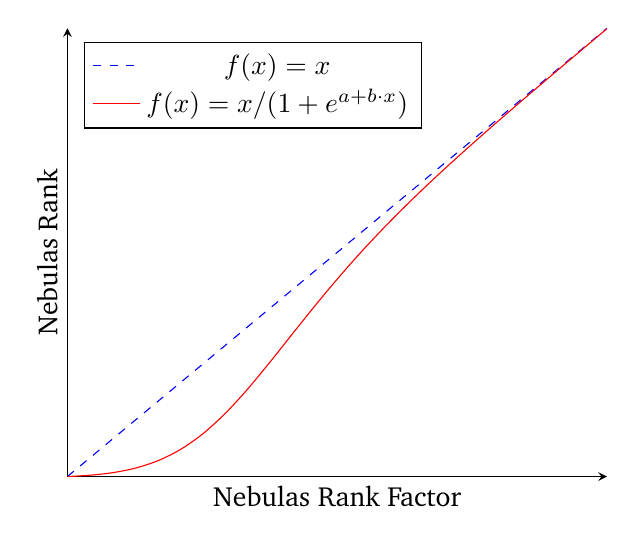
\begin{tikzpicture}[
    declare function={func(\x,\mu) = (\x / (1 + exp(\mu-\x)));},
    declare function={linefunc(\x) = \x;}
]
\begin{axis}[
    axis lines=left,
    enlargelimits=upper,
ticks=none,axis x line=bottom,axis y line=left,xlabel={Nebulas Rank Factor},
  ylabel={Nebulas Rank},
      legend pos=north west,
legend style={fill=none}
]
\addplot [dashed, domain=0:10, blue] {linefunc(x)};
\addplot [smooth, domain=0:10, red] {func(x,3)};
\addlegendentry{$f(x)=x$}
\addlegendentry{$f(x)=x/(1 + e^{a + b\cdot x})$}
\end{axis}
\end{tikzpicture}
\caption{The curve of the Nebulas Rank function \label{fig-nr}}
\end{figure}
\section{总结}
我们可以发现,区块链的共识和传统共识机制存在许多相似之处。例如对于区块一致性的达成本质上也是状态机复制,同时区块链共识在拜占庭环境下对安全性和活性的需求也并不能违背FLP定律。

但区块链相比传统分布式系统更为复杂,主要表现在以下几个方面。

\begin{itemize}
	\item 以比特币为代表的区块链系统摆脱了传统分布式系统的领袖-备份节点的设定,后者被认为是共识达成的瓶颈之一\cite{howard2019consensus}。在区块链系统中,出块节点负责发起对整个系统的状态更变,因此区块提议作为区块链共识机制中的重要部分被广泛研究,具体来说,理想的提议机制需要满足不可预测性以及合理出块频率。%尽管PoW由于能耗问题引起大量争议,但其仍被认为是目前最好的区块提议机制\footnote{https://zhuanlan.zhihu.com/p/52251671}。
	\item 区块链共识对于拜占庭容错的需求非常高,在大规模的异步网络下,应该优先保证安全性。同时,区块链共识需要保证已经达成一致的状态不会被改变(或者发生改变的概率非常低)。
\end{itemize}

与此同时,我们看到越来越多的研究关注于具有扩展能力(Scale-out)的区块链共识算法,在并没有严谨定义的Layer 1\&Layer 2概念中,分片技术(Sharding)被认为属于Layer 1机制,而闪电网络(Lightning Network)、状态通道(State Channel)等技术被认为属于Layer 2机制\footnote{https://lucidity.tech/layer-2-blockchain-technology/}。上述技术并不对区块链共识产生本质上的影响,我们将在后续工作中进一步阐述。



\newpage
\begin{appendices}
\section{对PoW的进攻方式}
自比特币被提出同时成为最具影响力的区块链项目以来,对其核心的PoW协议的种种进攻方式的提出,以及相应的对策,相应安全性的分析从未停止过。目前大家熟知的就有“51\%攻击”(主要能实现“双花攻击”),以及2015年Eyal等人提出的“私自挖矿”攻击等等,同时还存在着鲜为人知甚至潜在的尚未被发掘的进攻方式。作为共识的设计者,深入了解此类进攻方式的工作原理及影响,并分析相应的对抗策略,无疑能为所设计共识的安全性提供极大帮助。

近期,Ren Zhang等人关于PoW进攻方式的研究的论文发表在安全领域顶级会议2019S\&P上(暂无引用链接)。这里我们以这篇论文为基础,简要概述其结论,并为本设计指导提出一些对PoW进攻方式见解与思考。

就目前而言最为广泛的进攻方式可大致分为两大类
\begin{itemize}
	\item 分叉攻击
	
	这类攻击方式就包括我们熟知的\textbf{双花攻击}:在攻击者$a$支付数字货币的交易$a\rightarrow b$被区块$B$打包,并且攻击者$A$获得实际(如线下收货)收益后,以$B$区块的父区块为根进行分叉产生新区块$B'$,同时$B'$包含攻击者将同一笔数字货币支付给其小号的交易$a\rightarrow a'$,进而达到否定区块$B$及其中交易$a\rightarrow b$的目的。结果$b$没能收到款但$a$收到了货。
	
	通常认为双花攻击需要攻击者达到全网$50\%$以上算力。
	
	同时也包括所谓的\textbf{私自挖矿攻击}。当攻击者挖出新区块后,并不选择立即公布这个区块,而是私自在新区块上继续挖矿并不断加长更新,即,维护自己的一条“私链”。当私链长度大于主链长度时,攻击者选择一直在私链挖矿。只有当私链长度等于主链长度时,攻击者才选择公布其私链并期望私链能赢得之后的算力竞争。结论表明只要攻击者算力大于全网的$1/3$,私自挖矿即可以让攻击者有利可图。具体分析见原论文\cite{eyal2018majority}。
	
	私自挖矿可以和双花攻击进行结合,即先在主链进行交易后再公布私链用以否定主链交易。
	
	\item 定点攻击
	
	这类攻击有个专业名称叫feather-fork,最早见于比特币论坛上\footnote{https://bitcointalk.org/index.php?topic=312668.0}。
	
	此类攻击允许攻击者在拥有即使小于$50\%$算力的情况下完全隔绝任何来自某特定地址(即所谓黑名单,如Alice)的交易。具体操作如下:
	
	攻击者事先做出一个承诺(commitment\footnote{commitment是博弈论中一个重要概念。见https://en.wikipedia.org/wiki/Stackelberg\_competition}):我永远不会在任何包含来自Alice的交易的区块上进行挖矿。攻击者会一直遵循他所做的承诺。
	
	作为一个普通矿工,当他听到攻击者的承诺后,作为一个利益最大化的个体,他在打包交易的时候也不会包含任何来自于Alice的交易:如果他的区块包含了Alice的交易,那么在攻击者拥有算力为$\alpha$(全网百分比)的情况下,至少有$\alpha^2$的概率攻击者连续挖到两个区块,这两个区块将接在该矿工区块的父区块上,使该矿工挖出的区块成为孤块而丧失奖励。而矿工不打包Alice的交易仅仅损失少量交易费。其结果是,所有理性矿工都会隔绝Alice的交易,达成所谓定点攻击。一般而言$\alpha$越大能拉拢的普通矿工越多。
	
	造成定点攻击的原因在于理性矿工与协议矿工(reference miner)的区别:理性矿工总会最大化自己的利益,而协议矿工会至始至终按协议运作。定点攻击只有在协议矿工的比例少于$50\%$时才作效。
	
	\item 其他攻击(跳链,矿池)。
	
	跳链严格来说不是一种攻击:因为比特币的挖矿难度是根据2周内平均挖矿时间动态调整的,那么,很多大矿工大矿池可以选择在比特币难度较高的时候转去其他PoW公链挖矿,待比特币难度降下来(必然结果。因为矿工跳槽了,总算力减少)之后再回归比特币。来源见于Bitcoin-NG~\cite{eyal2016bitcoin}
		
	所谓矿池相关攻击不属于共识层面,是因为矿池的引入导致各式矿工行为。这里稍微介绍下仅供参考。
	
	Pool-hopping~\cite{rosenfeld2011analysis}: 类似,有的矿池是根据单位时间收益(出块奖励/挖矿时间)来分配奖励。那么,矿工可以在某矿池挖了一段时间没挖出矿后跳到别的矿池去挖矿,因为在原矿池继续挖即使挖出来了因时间太长收益也低。一般为达到平均时间的$43.5\%$即跳槽。
	
	派间谍(Miners' dilemma~\cite{eyal2015miner}):简单而言,矿池$A$可以派一部分矿工,所谓间谍,去矿池$B$挖矿,但是间谍挖到真正的矿不会提交给$B$矿池,只提交挖矿的证明。(提交share,难度为矿的千分之一)。相当于,间谍从$B$矿池领工资但不真正挖矿,工资分给$A$矿池的人。(当然$B$矿池也会向$A$矿池派间谍,形成一个类似囚徒困境的局面)。
\end{itemize}

文章接下来分析了某些著名的PoW项目针对这些攻击的安全性,同时提出了几项评价指标。这里不详细介绍。其重点结论在于,针对上述进攻安全性不能同时满足:存在一个安全性悖论:“rewarding the bad and punish the good”。具体而言,对于区块链分叉,一般存在两种处理方式:

\begin{itemize}
	\item 对所有分叉同给予同样奖励,所谓“reward-all”。举例包括fruitchain,EthPoW(叔块)等。此类项目由于分叉没有损失,会加剧分叉攻击。
	
	\item 对分叉进行惩罚,所谓“punishment”,如将出块奖励均匀分发给各个分叉。举例包括DECOR+,Bahack‘s idea。此类项目由于分叉损失过大,理性矿工会更加担心自己挖出的块成为孤块,进而加剧定点攻击。
	
	\item 还有一类叫做“reward lucky”。此类协议奖励某些区块,定义比较模糊。举例如Subchains,Botail。但是文章认为lucy不等于good,也不能达到效果。
\end{itemize}

所以,该论文给我们的思考在于,设计共识应达成上述安全性的一个平衡。

文章最后给出的共识参考建议也值得一提:
\begin{itemize}
	\item 设计的协议不应该太复杂。
	\item 不应只针对特定的攻击来进行安全性分析。(应全面考虑)
	\item 不应针对特定攻击者奖励进行安全性分析。(应全面考虑)
\end{itemize}
另外,文章指出安全性能基于下面几项要素得到提高
\begin{itemize}
	\item 网络环境更好
	\item (弱)全局时钟的存在
	\item 可信赖的第三方
	\item 责任外包制度
	\item 基于“Layer 2”的抗攻击手段。
\end{itemize}


\section{谜题选择}
谜题(puzzle)在PoW协议中扮演重要角色。通常,PoW协议规定只有解决给定谜题的矿工拥有出块权,是一种抵抗女巫攻击的有效手段。有文章指出PoW本质是通过谜题实现一个分布式时钟\footnote{https://grisha.org/blog/2018/01/23/explaining-proof-of-work/}。

谜题的选择同样也面临各式各样的取舍:
\begin{itemize}
	\item 谜题固然需要一定的难度来防止女巫攻击,但另一方面,有研究表明对于任何算力竞赛模型,高难度的谜题存在马太效应,更容易造成大户垄断(51\%dominance)。
	
	\item 谜题的难度固然需要动态调整以适应不断升级的算力,但另一方面,动态难度会造成跳链现象(见章节\ref{ch:attack})。同时,动态难度也会遭受所谓长程攻击(long-range attack),即攻击者从某远古区块开始一直以极低算力挖一条私链,因难度是动态的私链增长速率可以和主链一致,然后攻击者一定时间段突然加大算力,使私链长度大于主链。通常解决长程攻击的方式为矿工检测到分叉时,除简单的采取最长链原则外同时也要检测区块难度,以摒弃难度过低的链。
\end{itemize}

鉴于谜题在PoW协议中的重要作用,作为区块链共识设计者,了解包括比特币在内的多个PoW所采用的谜题及工作原理,优势劣势等,也是设计合理的PoW共识必不可少的一部分。

本章节主要针对Mimblewimble共识协议(Grin项目)所采取的谜题进行介绍并展开思考。该谜题名称叫cuckoo,发表在2015年FC上\cite{tromp2015cuckoo}。

比特币的挖矿工具经历了CPU,GPU,FPGA,ASIC四个阶段。现今有比特大陆等矿机公司已经本质上实现了比特币的算力垄断。而cuckoo旨在提出一种新的谜题,使得挖矿工具的更新停留在GPU这一步——只有1060以上显卡才能进行挖矿。

谜题的本质是验证(verification)与探索(proof attempt)的不对称性。比特币所采取的SHA256由于哈希函数的难逆性无疑符合条件。cuckoo采取的是随机图找环算法,通过引入内存带宽限制构建谜题的难度。具体步骤如下:
\begin{itemize}
	\item 图的生成。
	
	二部图的$N$个点已经给定,通过哈希函数随机生成二部图的$M$条边(大约$N/2$)。生成边的方式要满足一定的要求,可以理解为每条边是根据$(k,nonce)$的SHA512值决定,其中$k$为编号,$nonce$为矿工尝试的数字。验证时,一旦给出nonce则可还原出图中所有的边。
	
	\item 谜题目标。
	
	给定一个图,矿工需要给出一个长为$L$的环。验证时,一旦给出图以及$L$个点的编号,可以轻易验证环是否能形成。
	
	值得一提的是,从一个图里面寻找长为$L$的环是多项式时间可解的\footnote{$L$为偶数时,时间复杂度为$n^2$。$L$为奇数时,时间复杂度为$M(n)$,其中$M(n)$为计算矩阵乘法所需的时间复杂度。}。然而由于图的生成是完全随机的,且每个图大概率不存在长为$L$的环,故矿工仍然需要暴力搜索。
	
	\item 找环推荐算法。
	
    文章推荐算法包含两部分。
    \begin{itemize}
    	\item 减支部分
    	
    	所谓减支本质上是完成一个拓扑排序问题:去掉所有度数为1的以及相邻的边,重复上述过程直到所有点的度数$\geq 2$。由于上述减支过程需要存储每个点的度数,故需要进行大量内存读取。这就是该谜题能引入内存带宽限制的原因。
    	
    	文章同时也提出了其他的减支算法,$BFS(L)$和$BFS(L/2)$,能避免对每个点都记录信息,但会消耗更多的时间,是一种时间和存储的平衡(TMTO,time-memory trade-off)
    	
    	\item 找环部分。
    	
    	文章推荐的找环算法维护一个有向图森林,以类似并查集的方式将边逐条加入。一开始,所有孤立点各自都是一座森林。一旦一条边加入,如果两个端点属于两个不同森林,则将两个森林合并,通过维护森林中边的指向与每个节点的root值。当且仅当新加入边的两个端点属于同一森林时,则必存在一个环,可根据有向图路径找到该环并确定长度。
    	
    	值得一提的是,如果找出来环的长度不为$L$,则忽略该条边继续上述操作。这样虽然可能导致有的长为$L$的环被漏掉,但这种情形概率不高,作为一种概率性的算法仍能保证高效性\footnote{高效概率性算法在实际运作中比比皆是。一个经典的例子是质数判定问题$Prime()$。有研究已经证明该问题是多项式时间可解,但时间复杂度仍然很高。实际运行时人们仍然选择用费马小定理进行判断。后者不能保证$100\%$正确但更快。另一个例子是线性规划问题,虽然已被证明椭圆算法能在多项式时间解决,但人们更多的还是采用单纯形法,后者不能保证多项式时间解决,但实际平均运行时间往往更低。}。
    \end{itemize}
\end{itemize}	
文章推荐的数据规模$N=2^{25}+2^{25}$,$L=42$

文章接下来给出了很多实验图表。这里不一一列出,仅简要介绍结论。
\begin{itemize}
	\item 计算哈希函数的时间开销随着节点规模增大而减小,最终低于$15\%$。(大部分时间用于找环)
	\item 存在$42$环的概率在$M/N>1/2$时剧烈增长。
	\item 内存的读开销随着已尝试nonce的百分比指数级上升,但写开销持平。
	\item 存在环的概率与$L$大约成反比。
\end{itemize}

总结:就目前而言cuckoo能限制矿机,但同时也需要考虑到新型矿机的可能性(如基于路由器的大带宽)。
\section{随机数的生成}
所有涉及委员会选举,权益证明的区块链都离不开随机数的应用。而区块链上的随机数与人们传统理解又有所不同:区块链本质是实现一个状态机复制的问题,故要求所有的节点以相同条件生成随机数都会得到同样的结果,这就杜绝了以物理方式生成随机数的可能(包括宇宙辐射,random.org,等等)。

区块链上的随机数基本要求是不可预测性与可验证性,否则不能满足区块链的需求:首先,出块权这种不能被预测,否则会引发一系列问题(DDOS攻击)。同时,区块链一切算法是公开的,不存在一个中心节点秘密生成随机数。这就要求所有人都能验证随机数的合法性。	

此章节以Randao白皮书为参考\footnote{https://www.randao.org/whitepaper/Randao\_v0.85.pdf},指出随机数(或随机种子)生成需要权衡的几个问题:

\textbf{最后演员问题 “last actor problem”}

当随机数的生成需要多人合作时,最后一个做出行动的成员在其他成员行动后可以预知随机数的值,而其余成员因缺少最后行动者的行动无法获知,造成信息不对称。而一旦最后行动者发现随机数对自己不利,他可以选择拒绝行动。

Algorand生成随机种子的方法为,以上一轮出块者的VRF函数(可验证)作为下一轮的随机种子。因为Algorand算法无法预测出块者,故能满足不可预测性。

但我们认为Algorand中的算法存在最后演员问题:出块权是根据账户优先级决定的,而优先级来源于每个出块者的VRF,需要进行广播。而一旦一个矿工已经接受到所有其他矿工的广播,然后发现自己的优先级是最高的,他可以提前知道自己是出块者(只要他在限定时间内广播并且所有节点正常运作)并知道下一轮随机种子。进而他也可以选择不出块来改变区块链的结果(outcome)。

Dfinity和randao采用BLS($(t,n)$门限签名)方式生成随机数。因为在得到$t$个独立签名之前无法恢复出组签名,故所有用户均无法预测组签名值,满足不可预测性。但是也存在最后演员问题:当一个用户收到$t-1$个独立签名之后,他可以提前恢复出组签名,获取随机种子,进而也可以根据结果选择拒绝运作。当然,只要剩余$n-t+1$个人不都怎么做,组签名还是能成功运作。所以,该算法能抵御非法成员少于$n-t+1$的最后演员问题,且$t$越大越难抵御。

但是,如果$t$太小的另一个明显的问题是,任何$t$个成员可以共谋,无视剩余$n-t$个成员进行所有组签名操作。故BLS能抵抗$\min\{ n-t,t-1\}$个非法成员。所以一般选取$t=(n-1)/2$。

同时,BLS的另一个问题是生成的随机种子随机性不能满足。所谓随机性指任何一个对手无法在多项式时间内区分算法返回的随机数和一个真正的随机数。Algorand的VRF签名能满足随机性要求,然而门限签名由于限制颇多,并不能理论保证返回结果的随机性。Randao采取的方式是选取多个组串行进行签名,即,前一组的输出结果作为下一组的输入进行门限签名,但仍没有理论证明。

	


\section{投票系统}
\label{ch:voting}
目前关于电子投票(Electronic Voting)的研究中\cite{kiayias2002self},除去传统的隐私性(Privacy)、公平性(Fairness)和健壮性(Robustness)需求,理想的电子投票还需要满足如下要求:
\begin{itemize}
	%\item 隐私性:
	%\item 健壮性:
	%\item 公平性:
	\item 可校验性(Universal-Verifiability):任何第三方都可以验证最后的投票结果是否正确统计了合法选票\footnote{另有原子可校验性描述仅投票者可以验证投票结果是否正确统计了合法选票。};
	\item 无收据性(Receipt-Freeness):投票者无法向第三方证明其所投的选票内容;
	\item 无争议性(Dispute-Freeness):任何第三方都可以验证协议的参与方是否正确执行了协议;
	\item 自计票性(Self-Tallying):任何第三方可以进行计票,而不需要可信第三方或者投票者的参与;
	\item 完善保密性(Perfect Ballot Secrecy):假设存在$n$个选民,任何$t$个($t<n$)投票者的投票结果只有剩余$n-t$个投票者串通起来才能知道。
\end{itemize}

而对于共识机制中的投票系统,由于不存在可信的第三方机构,每个验证节点既是投票者也是计票者\textcolor{red}{(即所谓的"all voters are talliers")},因此其必须满足可校验性和自计票性。\textcolor{red}{论文\cite{kiayias2002self}指出在大规模的投票系统中,并不需要满足完善保密性。}

现有大多数基于投票的共识机制都无法满足无收据性和无争议性,具体地来说,对于拜占庭验证节点,虽然无法伪造或篡改其他人的消息\footnote{通常而言,我们认为现有的签名算法可以保证信息无法篡改或者伪造。},但仍可能出现如下恶意行为:

\begin{itemize}
	\item 恶意投票:恶意验证者不发布任何投票或者对其他验证者发布不同的投票,例如对部分验证者发布$\langle pk_i,sign_{sk_i}(t,h(B_1),\pi_i) \rangle$,而对另一部分验证者发布$\langle pk_i,sign_{sk_i}(t,h(B_2),\pi_i) \rangle$,$B_1 \neq B_2$。
	\item 割裂网络:在采用Gossip协议传输的网络中,恶意节点可能在收到其他节点的投票后不向其他节点转发该信息,导致原有投票信息无法广播到所有节点。
	\item 共谋:恶意节点在投票前或者投票过程中得知其他验证者身份,从而贿赂其他验证者使其投票决策发生变化。
\end{itemize}

\textcolor{red}{作为分布式系统,区块链中所有验证节点通过P2P方式进行通信,因此任何节点在投票过程中都无法检验其他节点是否正确执行协议,即在投票过程中无争议性无法保证。}\footnote{尽管Casper通过Slash机制实现了检点的互相监督,但恶意行为被发现是基于交易已经上链的前提。}在这种情况下,恶意投票和割裂网络将变得可行。这两种行为会导致决策无法收敛,从而影响共识的活性。%目前的投票共识往往通过监督检举的方式来减少恶意投票和割裂网络行为\cite{buterin2017casper}。

共谋行为则违背了无收据性,\textcolor{red}{现有大部分投票共识都没有考虑拜占庭节点的共谋行为}并且假设系统中拜占庭节点比例低于某个阈值(例如三分之一),而实际上,由于共谋行为的存在,系统中拜占庭节点比例会更高。
\section{匿名性}
通常,委员会选举,投票过程,包括某些共识过程都对匿名性有要求。匿名性能抵御贿赂现象,DDOS攻击,打击报复等等。Algorand通过每次抽取不同的委员会成员来投票的方式实现了部分的匿名性。

(未完待续)
\end{appendices}
%\printbibliography
\newpage
\bibliography{./reference}

\end{document}
